%中間審査概要テンプレート ver. 3.0

\documentclass[uplatex,twocolumn,dvipdfmx]{jsarticle}
\usepackage[top=22mm,bottom=22mm,left=22mm,right=22mm]{geometry}
\setlength{\columnsep}{10mm}
\usepackage[T1]{fontenc}
\usepackage{txfonts}
\usepackage[expert,deluxe]{otf}
\usepackage[dvipdfmx,hiresbb]{graphicx}
\usepackage[dvipdfmx]{hyperref}
\usepackage{pxjahyper}
\usepackage{secdot}





%タイトルと学生番号,名前だけ編集すること
\title{\vspace{-5mm}\fontsize{14pt}{0pt}\selectfont ブロックチェーン技術を用いたマネジメント法の提案}
\author{\normalsize プロジェクトマネジメントコース 矢吹研究室 1442068 鈴木 博文}
\date{}
\pagestyle{empty}
\begin{document}
\fontsize{10.5pt}{\baselineskip}\selectfont
\maketitle





%以下が本文
\section{背景}

「ファイナンス」と「テクノロジー」を掛け合わせた「フィンテック」が,日本でも注目を集めている.金融と最先端の技術が様々な形で融合して作り出す新しい金融サービス,さらにその潮流や動向を総称してこのように呼称する\cite{fujitsu}.中でも世界的に流通が拡大している,ビットコインを始めとした「仮想通貨」がある.その「仮想通貨」が通貨として機能し,サービスが成り立つ上で非常に重要な技術と言われているのがブロックチェーンだ.

ブロックチェーンは,取引の履歴を記録するデータベースを分散的に管理する手法のことで,「分散型台帳」とも呼ばれる.ブロックチェーンは「仮想通貨」だけでなく他の分野への応用が始まっている.投資や土地管理,投票など,他の分野でも活用が試みられている.

Jack du Rose氏が運営するColony社は,ブロックチェーンを会社経営・マネジメントに応用し,インターネット上での組織の自律的な運営を試みている\cite{wired}.

\section{目的}

様々な分野で活用が広がるブロックチェーン技術を,マネジメントに応用した例を参考にプロジェクトマネジメント(以下,PM)学科において同技術を利用した際の利点・難点を研究したいと考える.複数人でのソフトウェア開発プロジェクトにおいて開発システムの分散型管理を行った際の利点と難点を調査し,より効率の高いマネジメントの遂行とプロジェクトの成功につながるよう役立てる.

\section{手法}

オープンソース「ブロックチェーン技術推進コミュニティ」であるHyperledgerを利用する.Hyperledgerによって提供されているオープンソースのブロックチェーン実装Hyperledger Fabricを利用し,プロトタイプを開発する.

\section{想定される成果物}

ブロックチェーン技術をPMに応用した際に得られる利点・難点をまとめ,推奨される使用法を一覧とする.ブロックチェーン技術を用い複数人でソフトウェア開発を行える環境を実装する.

\section{進捗状況}

ブロックチェーンで生成されるブロックの構造を理解した.チェーンの安全性を維持するため,1つ前のブロックのハッシュ値が新規生成されたブロックに含まれていることを確認し,図\ref{naivechain}の結果を得た.

%図の挿入
\begin{figure}[h]
\centering
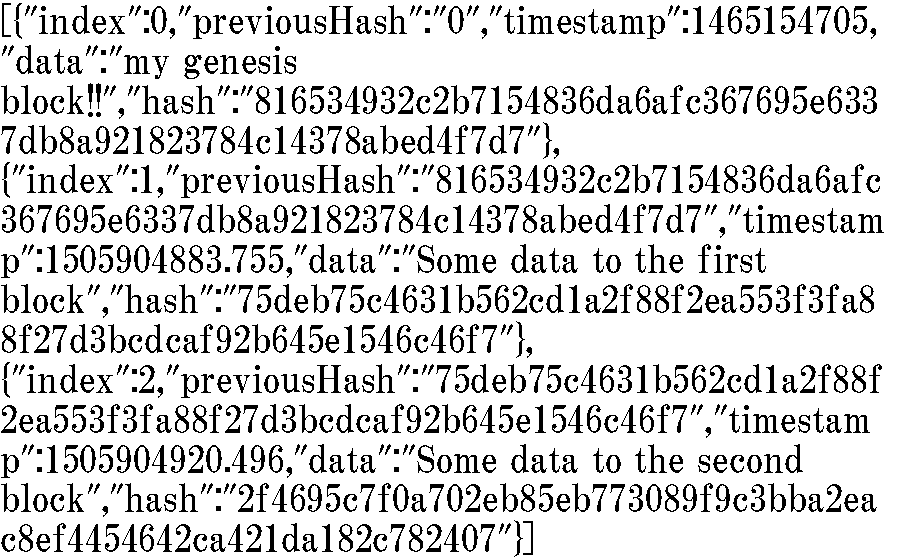
\includegraphics[width=5.8cm,clip]{chaincode.pdf}
\caption{NaiveChainを用いたブロック作成の実行結果}\label{naivechain}
\end{figure}

この他にHyperledger Fabricに付属する6つのサンプルを実行し,アカウントの作成とログイン,仮想通貨の送金と受取を実行した. 

\section{今後の計画}

Hyperledgerを用いて想定される成果物のプロトタイプ作成を開始する.利用が行えるようになった段階で研究室内にて稼働させ利点・難点をまとめたいと考える.

\bibliographystyle{junsrt}
\bibliography{biblio}%「biblio.bib」というファイルが必要.

\end{document}
